Dostarczony system składa się z kompilatora, programu do wysyłania binarnego pliku na zestaw startowy oraz procesora do uruchomienia na płytce FPGA. W razie gdyby użytkownik chciał samemu rozwijać dalej system lub po prostu go skompilować w poniższym rozdziale poza standardowym opisem kolejnych kroków podajemy również - na samym jego początku - jak zbudować kompilator z kodu źródłowego i jak uruchomić procesor na FPGA.
\section{Instalacja systemu i niezbędnych składników}
Podstawowym składnikiem potrzebnym do skompilowania haskellowej części projektu jest platforma Haskella. W skład jej wchodzą:
\begin{description}
  \item[Glasgow Haskell Compiler] \hfill \\
  otwarty kompilator i interaktywne środowisko funkcjonalnego języka Haksell 
  \item[Cabal build system] \hfill \\
  architektura do budowania bibliotek i aplikacji dedykowana dla Haskella
  \item[35 pakietów] \hfill \\
  Podstawowe i najczęściej używane moduły haskella
  \item[Narzędzia do profilowania i analizowania kodu] \hfill \\
  Interaktywne środowisko programowania, parsery i lexery haskellowego kodu, środowisko testowe
\end{description}

Platforme Haskella znaleźć można na oficjalnej stronie języka w zakładce Downloads(https://www.haskell.org/downloads).
Po zainstalowaniu platformy należy wywołać komendę \texttt{cabal install} w folderze \texttt{fpga-coprocessor/lang}. Komenda skompiluje kod źródłowy kompilatora i skopiuje go wraz z zależnościami do folderu \texttt{dist}.

Kolejnym wymaganym składnikiem jest środowisko Quartus II Web Edition potrzebne do kompilacji i uruchomienia projektu na zestawie startowym z układem fpga. Pobrać można je z centrum pobierania na stronie Altery (http://dl.altera.com).
Po otworzeniu projektu należy go skompilować klikając \textbf{Start Compilation} a następnie przesłać do urządzenia(\textbf{Programmer}\textgreater \textbf{Start}).

Ostatnim wymaganym programem jest kompilator języka C - GCC, the GNU Compiler Collection potrzebny do kompilacji programu wysyłającego plik binarny na zestaw uruchomieniowy i odbierającego wynik. Program skompilować można na przykład poleceniem 
\texttt{gcc send\_bin.c -o send\_bin}
\section{Konfiguracja sprzętu}
Do uruchomienia projektu potrzebny jest zestaw startowy z układem FPGA. Projekt rozwijany i testowany był na układzie \textbf{Terasic DE0-Nano z rodziny Cyclone IV} firmy Altera.

\begin{figure}[h]
\begin{center}
\includegraphics[scale=0.75]{images/de0-nano}
\caption{Zestaw startowy Terasic DE0-Nano Board}
\end{center}
\end{figure}

Komunikacja komputera PC z zestawem FPGA odbywa się za pomocą układu UART w związku z tym do przesłania pliku potrzebny jest \textbf{Konwerter USB-UART}. W projekcie wykorzytaliśmy Konwerter USB-UART PL2303 umożliwiający komunikacje pomiędzy interfejsami szeregowymi USB i UART widoczny w systemie jako wirtualny port COM.
\begin{figure}[!ht]
\centering
\includegraphics[scale=1]{images/usb-uart}
\caption{USB-UART PL2303 - wtyk USB}
\end{figure}
Pin GND konwertera należy połączyć z Pinem GND zestawu startowego(np. PIN12 JP1 lub PIN12 JP2). Pin TXD konwertera łączymy z pinem GPIO 11 natomiast Pin RXD z pinem GPIO 9.
\begin{figure}[!ht]
\centering
\includegraphics[scale=0.1]{images/full_connected}
\caption{Podpięty cały zestaw}
\end{figure}
Zestaw startowy należy podłączyć do komputera również poprzez dołączony kabel USB co umożliwi wgrywanie oprogramowania poprzez interfejs USB-BLASTER. Złącza RX i TX zaleca się oddzielić rezystorem o wartości 1K\ohm\space jednak z własnego doświadczenia możemy dodać, że nie jest to konieczne.
\section{Krótki kurs zaimplementowanego języka}
Planując język programowania wzorowaliśmy się na rozwiązaniach takich jak w ęzyku Ruby czy Python. Chcieliśmy by użytkownik nie musiał używać znaków takich jak średniki a równocześnie nie musiał zwracać uwagi na odpowiednie wcięcia i odstepy. Udało nam się uzyskać składnię która pozostając zawsze bardzo czytelną daje programiście możliwość formatowania kodu wedle własnego uznania.
\subsection{Znaki białe}
W zaproponowanym przez naz języku białe znaki (odstęp, nowa linia, wcięcie) są przez parser ignorowane.
Rozwiązanie takie daje możliwość formatowania kodu w sposób najbardziej elastyczny, zależny od potrzeb użytkownika. To samo wyrażenie można zapisać w wielu liniach na sposób możliwie czytelny lub jednej by otrzymać zwięzły, niewielki wizualnie kod.
Dla przykładu, przytoczone poniżej listingi zawierają ten sam program a różnią się jedynie formatowaniem:\\
\begin{lstlisting}[frame=single]
x:Int = if a
        then b = a * 2
             b + a
        else b = (a + 1) * 2
             b - 1
        end
\end{lstlisting}
\begin{lstlisting}[frame=single]
x:Int = if a then b=a*2 b+a else b=(a+1)*2 b-1 end
\end{lstlisting}
Jak widać nawet prostą instukcje warunkową \textbf{if} można zapisać w sposób bardzo czytelny jak w pierwszym przykładzie lub zwięzły - jak w drugim.
\subsection{Komentarze}
Dane są 2 rodzaje komentarzy - liniowe \texttt{\#} oraz blokowe \texttt{\string{\# ... \#\string}}\\
\begin{lstlisting}[frame=single]
# komentarz liniowy
{#
komentarz
blokowy
...
#}
\end{lstlisting}
Wzorując się na wielu innych językach dajemy użytkownikowi możliwość wykorzystania dwóch rodzajów komentarzy.
\subsection{Literały}
Będąc ograniczeni przez ilość bramek logicznych na układzie FPGA dostarczamy użytkownikowi 2 rodzaje literałów - liczby całkowite oraz wektory liczb całkowitych:\\
\begin{lstlisting}[frame=single]
1024
[1, 2, 4, 8, 16, 32, 64, 128]
\end{lstlisting}
Liczby całkowite jak i pojedyncze elementy wektora należą do przedziały [0,255].
\subsection{Zmienne, deklaracje zmiennych i przypisanie do zmiennej}
Każde wyrażenie w języku ma jeden z dwóch typów - \textbf{Vector} lub \textbf{Scalar}. Dodatkowo typ Vector parametryzowany jest jedną liczbą naturalną - długością wektora.
Przykłady deklaracji:\\
\begin{lstlisting}[frame=single]
# deklaracje zmiennych skalarnych
a:Int = 4
b:Int = 2*a

# deklaracje wektorow
x:IntVector[4] = [0,0,1,1]
y:IntVector[5] = [1,2,3,4,5]

# przypisania
a = 4
a = [1,2,3] # zle! a ma typ Scalar

z:Int #zle! przy deklaracji trzeba zainicjowac zmienna
\end{lstlisting}
Każda zmienna przed użyciem musi zostać zadeklarowana. Nie można zadeklarować zmiennej nie inicjalizując jej jednocześnie. Mechanizm ten chronić ma przed przypadkowymi błędami częstymi w innych językach.

\subsection{Operatory}
Język posiada 7 operacji wspierających obliczenia wektorowe:
\begin{description}
  \item[+] \textbf{Dodawanie} - operacja na 2 skalarach, lub 2 wektorach - wtedy element po elemencie
  \item[*] \textbf{Mnożenie} - operacja na 2 skalarach, lub 2 wektorach - wtedy element po elemencie
  \item[-] \textbf{Odejmowanie} - operacja na 2 skalarach, lub 2 wektorach - wtedy element po elemencie
  \item[/] \textbf{Dzielenie} - operacja na 2 skalarach, lub 2 wektorach - wtedy element po elemencie
  \item[?] \textbf{Iloczyn skalarny} - operacja na 2 równej długości wektorach - zwraca skalar
  \item[\%] \textbf{Modulo} - operacja na 2 skalarach, lub 2 wektorach - wtedy element po elemencie
  \item[rot90] - rotacja 4 punktów w przestrzeni dwuwymiarowej o 90 stopni względem punktu (256, 256)
\end{description}

Przykłady działania operacji:
\begin{lstlisting}[frame=single]
[2,3,4,5,6] + [1,2,3,4,5]   
   # =[3,5,7,9,11]
[1,2,4,8] - [1, 1, 2, 4] 
   # =[0,1,2,4]
[1,2,3,4,5,6] * [2,2,2,2,2,2] 
   # =[2,4,6,8,10,12]
[8,6,4] / [2,2,2] 
   # =[4,3,2]
[1,1,1,1] ? [2,2,2,2] 
   # =8
[64, 7, 24] % [8, 3, 16]
   # =[8, 3, 16]
rot90 [10,10,10,10,10,10,10,10] 
   # =[10, 246, 10, 246, 10, 246, 10, 246]
\end{lstlisting}
W powyższym kodzie po każdej operacji w następującej linijce podajemy zakomentowany wynik danego działania.
\subsection{Instrukcje warunkowe}
Instrukcja warunkowa ma postać:
\begin{center}
\textbf{if} \textit{expression} \textbf{then} \textit{expression\_block} \textbf{else} \textit{expression\_block} \textbf{end}
\end{center}
Przykład użycia:\\
\begin{lstlisting}[frame=single]
a:Int = 0
b:IntVector[4] = [0,1,2,3]
c:IntVector[4] = if a then b else b + [1,1,1,1] end
# c = [1,2,3,4]

d:IntVector[4] = if a+1 then b else b ? [1,2,1,2]
# niezgodne typy: w bloku pierwszym wektor, w drugim skalar 
\end{lstlisting}
Wartością zwracaną przez instrukcje jest ostatnie wyrażenie w pierwszym lub drugim bloku. Typem instrukcji jest typ ostatniego wyrażenia w obu blokach. Wynika z tego, że wartości zwracane przez oba bloki muszą mieć ten sam typ, by kod mógł zostać poprawnie otypowany. Blok pierwszy wykonywany jest jeśli wyrażenie warunkowe było różne od zera lub nie było wektorem zer, natomiast drugi w odwrotnym przypadku.
\subsection{Pętla loop}
Składnia pętli loop:
\begin{center}
\textbf{loop(} \textit{expression} \textbf{):} \textit{expression\_block} \textbf{end}
\end{center}
Przykład:\\
\begin{lstlisting}[frame=single]
term2:IntVector[8] = [1,1,1,1,1,1,1,1]
result:IntVector[8] = [0,0,0,0,0,0,0,0]

loop(254):
  result = result + term2
end
result
#expecting [254, 254, 254, 254, 254, 254, 254, 254] 
\end{lstlisting}
Pętla loop jako jedyna formuła w języku nie zwraca żadnego typu i służy do repetywnego wykonywania kodu podanego w ciele pętli. Jeśli ilość iteracji jest skalarem \textit{n} pętla wykonywana jest \textit{n}-krotnie. Jeśli wyrażenie wewnętrz okrągłych nawiasów jest wektorem to ilość powtórzeń instrukcji jest ostatnim elementem wektora.
\section{Kompilacja}
Po napisaniu programu użytkownik musi skompilować go do binarnej reprezentacji gotowej do wysłania na FPGA. Proces kompilacji może zostać zakłócony przez błędy syntaktyczne i semantyczne kodu. Kompilator może zwrócić też informacje o niepowodzeniu jeśli przewidzi, że kompilowany kod z pewnych powodów może nie zostać poprawnie uruchomiony na FPGA.
\subsection{Użycie kompilatora}
Do kompilacji należy użyć programu \textit{compilator} napisanego w haskellu i wygenerowanego w folderze \textit{dist/}(patrz 1.1). Kompilowany plik powinien znajdować się w aktualnym folderze i mieć nazwę \textit{example}.
Podczas kompilacji na ekran wypisane zostaną informacje o kolejnych etapach pracy, drzewo syntaktyczn programu, wygenerowany kod asemblera oraz użyte w programie stałe.
\begin{figure}[!h]
\centering
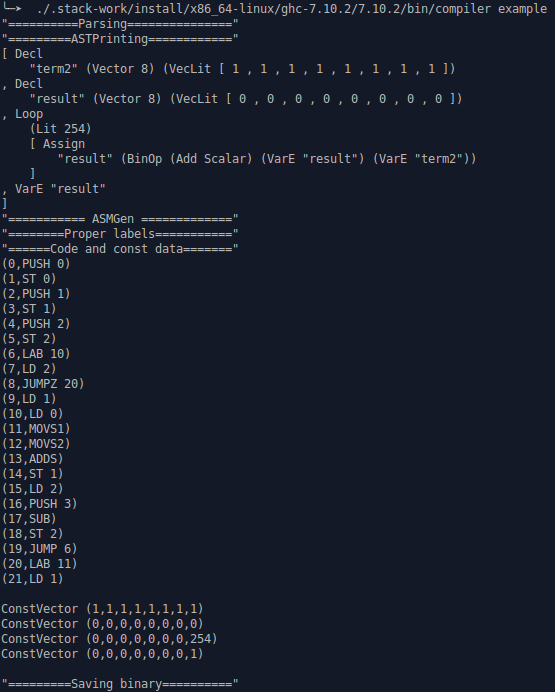
\includegraphics[scale=0.75]{images/kompilator}
\caption{Kompilacja programu}
\end{figure}\clearpage
Jeśli kompilacje przebiegnie poprawnie w bieżącym katalogu zapisany zostanie wygenerowany program.

\subsection{Możliwe błędy}
Proces kompilacji może zostać przerwany przez następujące błędy:
\begin{description}
  \item[Address of JUMP too big]\hfill \\
       Błąd wewnętrzny kompilatora - rozmiar kodu jest na tyle duży, że numer pewnej linijki nie zmieści się w rejestrze na FPGA.
  \item[Address of Push, Load or Store too big] The second item\hfill \\
       Kolejny błąd kompilatora - duży kod powoduje, że adres binarny zmiennej jest większy niż przewiduje architektura procesora.
  \item[No more address space for new variables] \hfill \\
       Błąd wynikający z dobranych rozmiarów pamięci na FPGA - nie ma już miejsca na kolejną zmienną w pamięci.
  \item[Assigning to non-existing variable]
       Próba przypisania do niezadeklarowanej wartości. Na przykład, w podanym poniżej programie użytkownik przypisuje wartość do niezadeklarowanej zmiennej a.
\begin{lstlisting}[frame=single]
a:Int = 2
\end{lstlisting}
  \item[Wrong type of X]\hfill \\
      Niezgodność typów podczas deklaracji zmiennej. Przykład - do zmiennej typu \textbf{Int} przypisanie wartości       \textbf{IntVector[5]}:
\begin{lstlisting}[frame=single]
a:Int = [1,2,3,4,5]
\end{lstlisting}  
  \item[X and Y differ] \hfill \\
      Częsty błąd wielu operacji binarnych. Próba np. przemnożenia 2 wektorów o różnych rozmiarach:
\begin{lstlisting}[frame=single]
[1,2,3,4,5] * [1,2]
\end{lstlisting}       
  \item[Rotation vector needs exactly 8 elements] \hfill \\
      Błąd operacji \textbf{rot90}. Wymaga ona współrzędnych 4 punktów w 2 wymiarach podczas gdy użytkownik podaje inną ilość.
\begin{lstlisting}[frame=single]
rot90 [100, 100, 230] # error!
\end{lstlisting}       
  \item[Empty statement block in if structure] \hfill \\
      Użytkownik nie wpisał żadnego wyrażenia do któregoś z bloków pętli.
\begin{lstlisting}[frame=single]
x:Int = if 0
        then # error!
        else
            2 * 5
        end
\end{lstlisting}        
  \item[Then and else returns different structs] \hfill \\
       Typ bloku \textbf{then} i \textbf{else} powinien być taki sam. W innym wypadku system sprawdzania typów nie zezwoli na kompilacje.
\begin{lstlisting}[frame=single]
x:Int = if 0
        then 
           [1,2,3]  # Vector[3]
        else
            2 * 5   # Scalar
        end
\end{lstlisting}   
  \item[Variable X undeclared] \hfill \\
      Użyto zmiennej która nie została zadeklarowana.
\begin{lstlisting}[frame=single]
x:Int = a * 2 # error!
\end{lstlisting}   
  \item[Loops dont return values] \hfill \\
     Użytkownik próbował przypisać pętle do zmiennej.
\begin{lstlisting}[frame=single]
y:Int = 0
x:Int = loop(5): # error!
           y = y + 1
        end  
\end{lstlisting} 
  \item[Variable X already declared] \hfill \\
      Podwójna deklaracja zmiennej.
      \begin{lstlisting}[frame=single]
y:Int = 0
y:Int = 1
\end{lstlisting} 
  \item[Cannot assign X to Y of type]\hfill \\
    \begin{lstlisting}[frame=single]
x:IntVector[5] = [1,2,3,4,5] ? [1,2,3,4,5]
\end{lstlisting} 
  Niezgodność typów przy przypisywaniu do zmiennej.

\end{description}

\section{Wysyłanie programu i odbieranie wyników}
Skompilowany kod zapisywany jest w binarnej reprezentacji do pliku \textit{binary}. Jest on gotowy do wysłania na płytkę FPGA. Służyć do tego może poprzednio skompilowany program \textit{send\_bin}.
\begin{center}
./sendbin binary
\end{center} 
Po wysłaniu programu na zestaw startowy zostanie on wykonany, a następnie na ekranie wyświetli się wynik programu.
\begin{figure}[H]
\centering
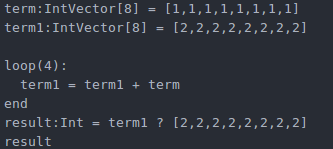
\includegraphics[scale=0.75]{images/exec1}
\caption{Kod źródłowy}
\end{figure}
Pierwszym krokiem jest napisanie poprawnego programu - np. paru iteracji w pętli i obliczenia iloczynu skalarnego.
\begin{figure}[H]
\centering
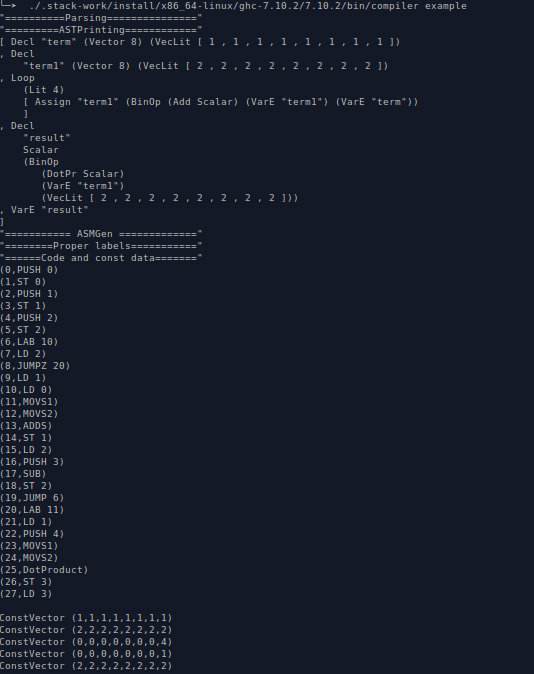
\includegraphics[scale=0.75]{images/exec2}
\caption{Kompilacja kodu}
\end{figure}
Następnie kod należy skompilować. Jeśli kompilator nie zaraportował żadnego błędu wygenerowany zostanie odpowiedni plik programu.
\begin{figure}[H]
\centering
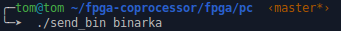
\includegraphics[scale=0.75]{images/exec3}
\caption{Wysyłanie kodu na urządzenie}
\end{figure}
Jeżeli urządzenie zostało poprawnie podpięte do komputera(tak jak podano w rozdziale 2.2) program zostanie przesłany na FPGA poprzez wirtualny port COM.
\begin{figure}[H]
\centering
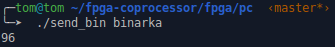
\includegraphics[scale=0.75]{images/exec4}
\caption{Odbieranie wyniku}
\end{figure}
Po przeprowadzeniu obliczeń procesor odeśle wynik a program z którego dane zostały wysłane - odbierze go i wypisze na ekranie.